\documentclass[a4paper,11pt]{book}
\usepackage[margin=2cm]{geometry}		
\usepackage[thinfonts]{uglix2}
\usepackage{array,numprint}
\newcommand{\tabstrut}{\vrule height 1.25em depth 0.5em width 0pt}
\begin{document}
\chapter*{\large Interaction entre l'homme et la machine sur le web \\[-1em]\fontsize{35pt}{42pt}\selectfont Interaction client-serveur avec Flask}

\double
{
	Précédemment nous avons créé un formulaire. Celui-ci ne fonctionne pas car il essaie d'envoyer les données collectées sur un site qui n'est pas 
	le bon.\\
	Lorsqu'un utilisateur surfe sur le Web avec un ordinateur (une tablette ou un smartphone), les interactions avec un site se passent comme sur le 
	schéma ci-contre : le site consulté est hébergé sur un \textit{serveur distant} auquel on accède grâce à son \textsc{URL} (\textit{Uniform 
	Resource Locator}, l'adresse du site). Plus le nombre de consultations simultanées du site est grand, plus le serveur doit-être puissant pour 
	pouvoir répondre aux demandes et traiter les informations.
}
{
	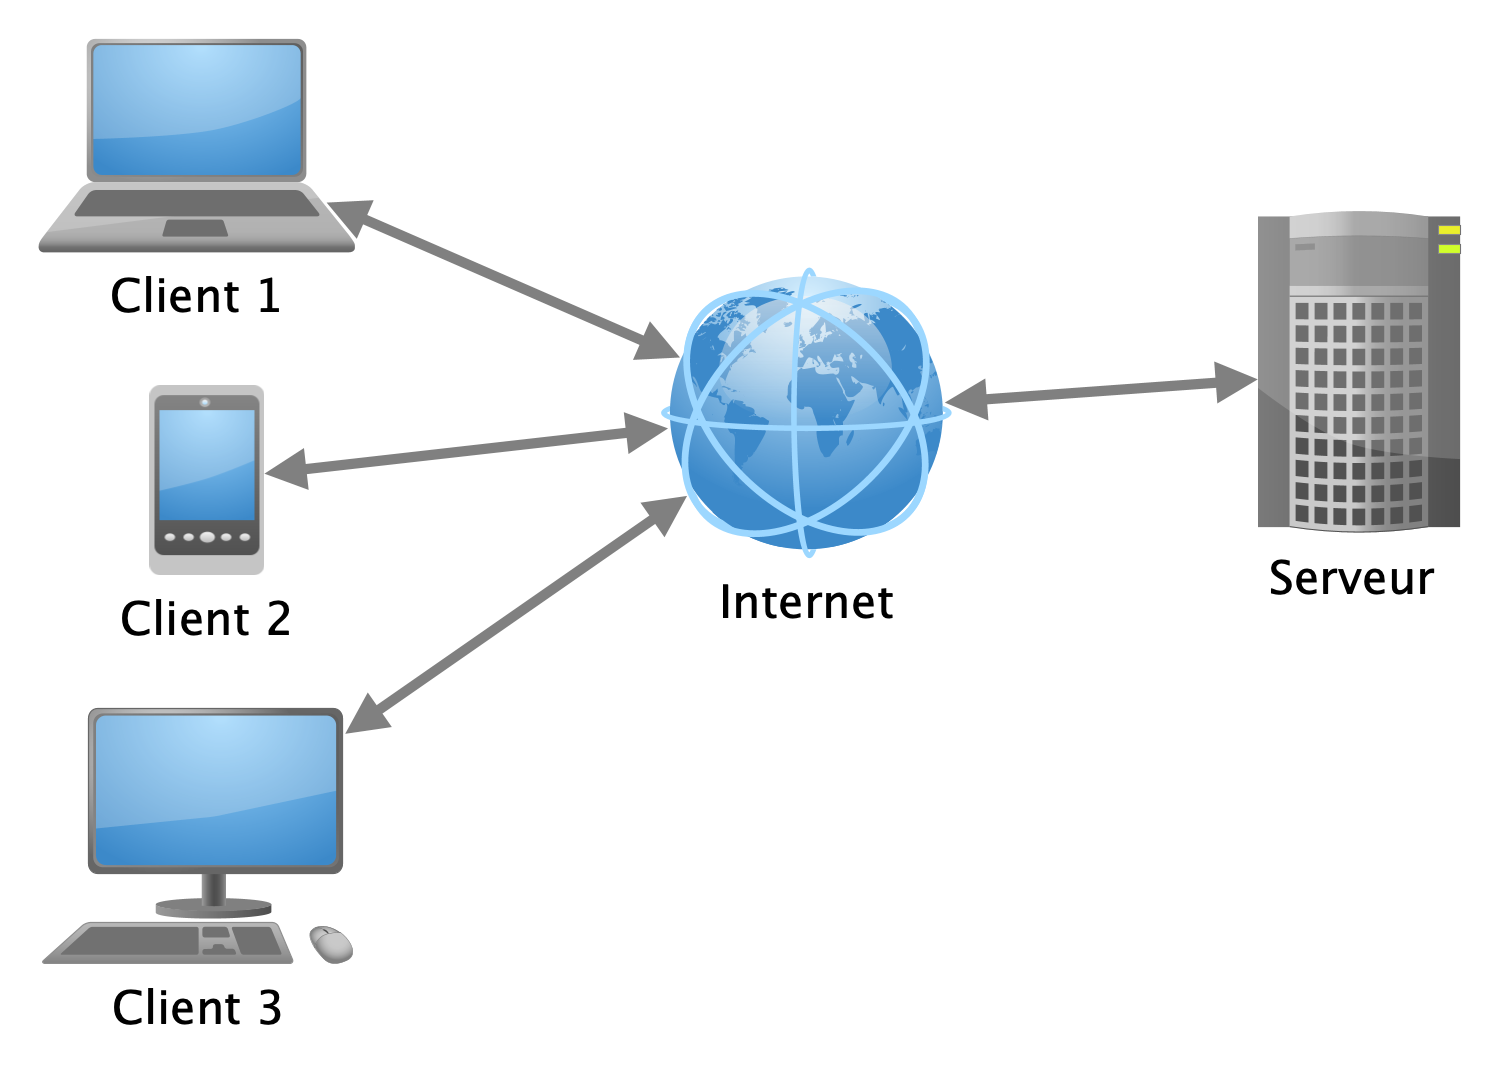
\includegraphics[width=6cm]{img/schema_web.png}
}{6cm}\\[1em]

\double{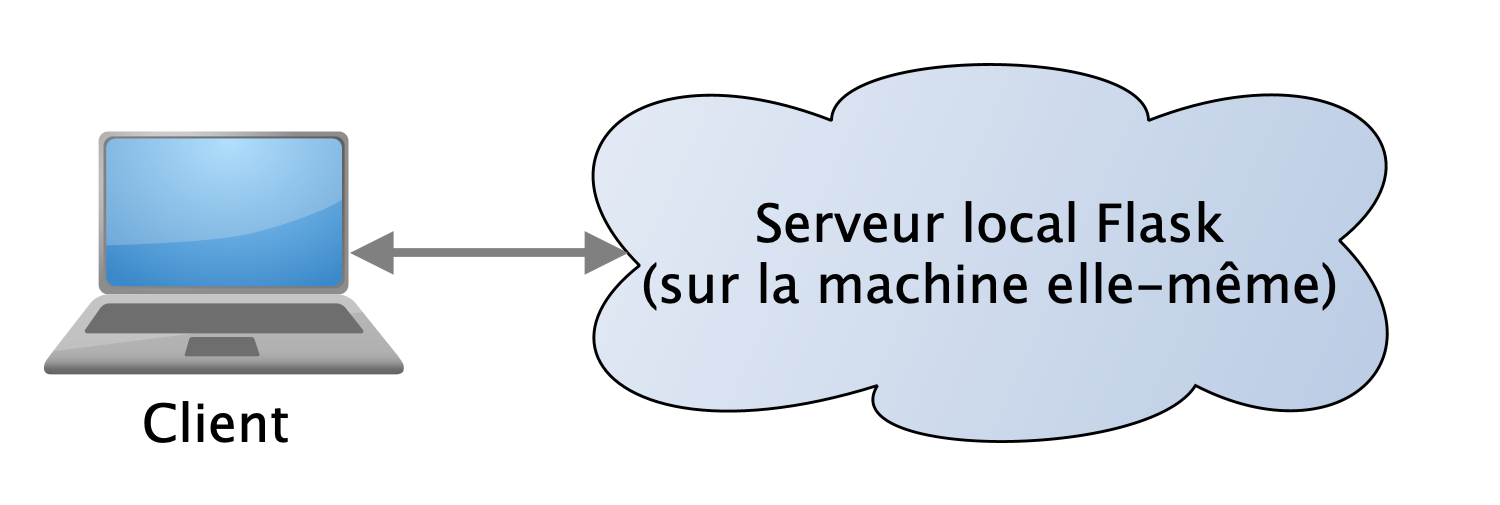
\includegraphics[width=6cm]{img/schema_local.png}}
{
Nous allons simuler la situation précédente sans recourir à un serveur distant : nous allons créer un \textit{serveur local}. Dans beaucoup de 
situations, le serveur (local ou distant) produit des pages \textsc{html} et traite les informations en utilisant le langage \textsc{PHP}.\\
Cependant nous pouvons aussi nous servir de \textsc{Python} pour faire la même chose, à l'aide de la bibliothèque \tw{Flask} !}{11cm}
\begin{center}

\includegraphics[width=4cm]{img/Flask.png}
\end{center}
Pour travailler avec \tw{Flask}, on va utiliser un \textit{environnement virtuel} sous \textsc{PyCharm}. Pour créer un tel environnement, regarde la vidéo suivante :\\

\url{https://youtu.be/uyctvyt0a8s}

\section*{Un exemple minimal de soumission de formulaire avec Flask}

Fabriquons un site très simple : on accède à la page \tw{index.html} et on remplit le formulaire, puis à l'envoi du formulaire, une page 
\tw{resultat.html} est affichée, qui exploite la donnée soumise \textit{via} le formulaire.\\

Il y a donc un fichier \tw{index.html}.
\begin{modulbox}{vertfonce@color}{Code HTML}
\inputminted{html}{flask_minimal/templates/index.html}
\end{modulbox}




Tu peux remarquer que le formulaire envoie les données à \url{http://localhost:5000}, c'est à dire à lui-même (c'est ce que veut dire \tw{localhost}) 
et sur le port 5000 (car \tw{Flask} est configuré comme cela par défaut).

Voici le fichier \tw{resultat.html} :


\begin{modulbox}{vertfonce@color}{Code HTML}
\inputminted{html}{flask_minimal/templates/resultat.html}
\end{modulbox}

Il faut comprendre que  \tw{\{\{nom\}\}} fait référence la variable \tw{nom} de la balise \htmlinline{<input>} de la page \tw{index.html}.\\

Il nous reste à connecter ces deux éléments en mettant en place un serveur \tw{Flask} et c'est là que \textsc{Python} intervient.

\pythonfile{flask_minimal/views.py}

Pour coordonner tout cela il faut \\
\double{\begin{enumerate}[--]
	\item 	Créer un répertoire pour mettre le projet (j'ai appelé le mien \tw{flask\_minimal});
	\item 	créer le fichier \textsc{Python} \tw{views.py};
	\item 	créer un répertoire appelé obligatoirement \tw{templates};
	\item  	créer dans ce répertoire les fichiers \tw{index.html} et \tw{resultat.html}.
\end{enumerate} 
}
{\includegraphics[width=5cm]{img/arborescence_flask.png}}{5cm}

\section*{À toi de jouer}

Tu vas reprendre le formulaire que tu as crée à l'activité \og produire un formulaire\fg{} et t'en servir comme base d'un petit projet \tw{Flask}.

\begin{exercice}[]
Crées une application web avec \tw{Flask} qui utilise ton formulaire comme point de départ : tu pourras renommer cette page \tw{index.html}. Il faudra bien veiller à modifier la balise \htmlinline{<form>} comme ceci :\\

\htmlinline{<form action="http://localhost:5000/resultat" method=post>}\\

Ensuite tu pourras par exemple analyser la date de naissance de l'utilisateur \textbf{dans le fichier views.py} et en fonction du résultat afficher une page \tw{mineur.html} ou bien  \tw{majeur.html}.\\
C'est à toi d'imaginer comment à l'intérieur du fichier \tw{views.py} tu peux traiter les informations du formulaire pour dynamiser ton exemple de site...
\end{exercice}
\end{document}